\chapter{Support Vector Machine }
\label{chapter:SVM}
\section{簡介}
\label{sec:SVMIntroduction}
SVM屬於一種監督式學習演算法,主要的目的是在特徵空間中,盡可能找到一個超平面使其能夠以最大間格把兩個類別區隔開來。
如圖\ref{fig:SVMBestSeparte}所示, \(H_1\)與\(H_2\)都能將兩個類別分離,但 \(H_1\)與最近的資料點間隔較小,如果資料集中有其他雜訊點, \(H_1\)很容易將其分類錯誤;而 \(H_2\)則能以較大的間隔區隔兩個不同類別,因此當資料集中有其他雜訊點,還是能須利將其分類。因此\(H_2\) 屬於比較好的分類器。

SVM除了可以處理線性分類問題如圖\ref{fig:SVMBestSeparte},同時也能解決非線性分割的問題如圖\ref{fig:LinearUnseparable}。利用核函數使低維度線性不可分的樣本映射到高維度,使得原本非線性可分的資料,變成可線性分割的資料,使SVM能在高維空間中建構超平面如圖\ref{fig:Hyperspace}所示,進而將原始數據進行分類。
%%\begin{equation}
%%	\label{eqn:SVM}
%%	_{w,\delta_i}^{min}\frac{1}{2}W^TW+C\sum_{i=1}^{n}\delta_i
%%\end{equation}
%%其中 w 為超平面的法向量,$\delta_i$超平面的容忍邊界參數,值越大容忍範圍越大,C 為調整容忍邊界參數的權重。
%%

\begin{figure}[H]
	\centerline{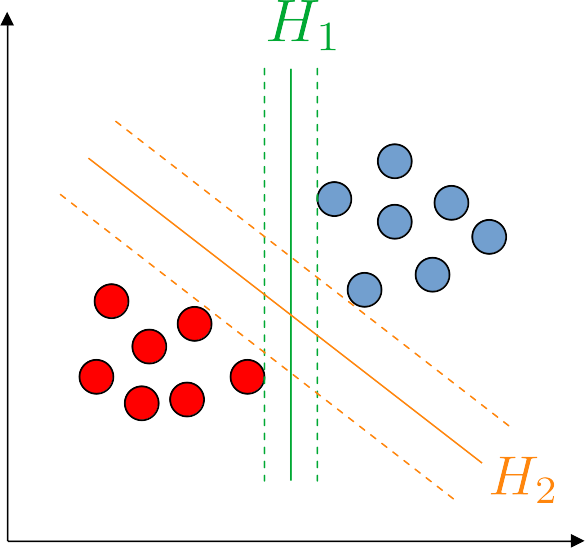
\includegraphics[height=5cm]{./pic/PnmhVqej.png}}
	\caption{資料集中不同的分割線}
	\label{fig:SVMBestSeparte}
\end{figure}

\begin{figure}[H]
	\centerline{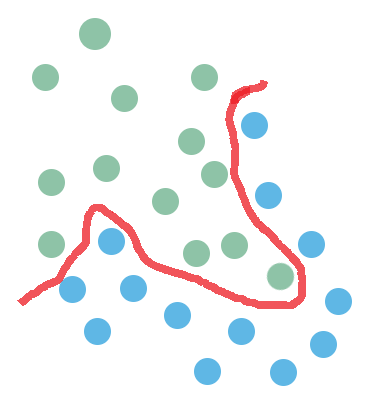
\includegraphics[height=5cm]{pic/unlinear.PNG}}
	\caption{線性不可分示意圖}
	\label{fig:LinearUnseparable}
\end{figure}

\begin{figure}[H]
	\centerline{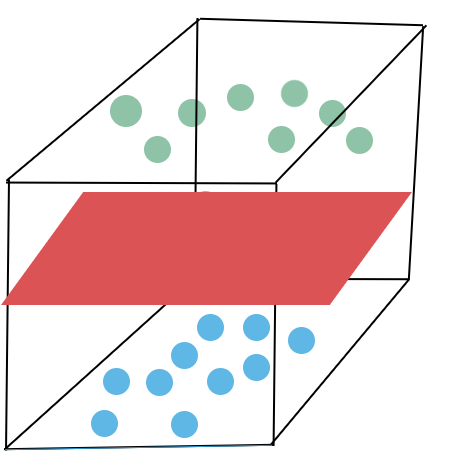
\includegraphics[height=5cm]{pic/over space.PNG}}
	\caption{超空間示意圖}
	\label{fig:Hyperspace}
\end{figure}

\section{演算法參數定義與流程}
以下說明演算法的推導流程。

\subsection{參數定義}
考慮線性可分的資料集如下:
$$(\mathbf{x_1},y_1),(\mathbf{x_2},y_2),...,(\mathbf{x_i},y_i),...,(\mathbf{x_n},y_n)$$

\begin{itemize}

	\item
	      \(\mathbf{x_i}\),表示其中一筆資料集,有d個元素,即 \(\mathbf{x_i}\in R^d\) 。\(y_i\),為資料的類別, \(y \in +1,-1\), \(y_i =+1\)表示\(\mathbf{x_i}\)為正類別,\(y_i =-1\)則表示\(\mathbf{x_i}\)為負類別。

	\item
	      \(\mathbf{w}\)與\(b\),分別表示超平面的法向量與截距,方程式為 \(\mathbf{w^Tx}+b=0\)。法向量指向的一側為正類,另一側為負類。
\end{itemize}

\subsection{流程}

\begin{itemize}
	\item
	      圖\ref{fig:SVMIllustrate}中有三個互相平行的超平面。
	      如\ref{sec:SVMIntroduction}節所述,SVM的目的是盡可能的找出最大間隔超平面,因此先選擇分離兩類數據的兩個平行超平面,使得其之間的距離盡可能越大越好。其中兩個超平面間範圍內的區域稱為「間隔(margin)」,最大間隔超平面是位於它們正中間的超平面。
	      \begin{figure}[H]
		      \centerline{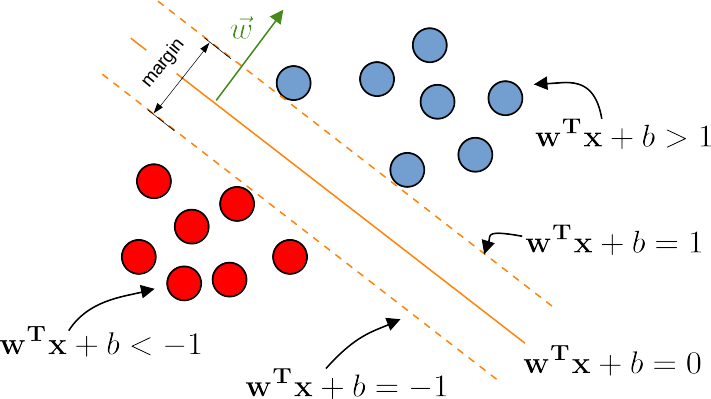
\includegraphics[height=6cm]{./pic/kq2oRLsT.png}}
		      \caption{SVM說明}
		      \label{fig:SVMIllustrate}
	      \end{figure}

	\item
	      由兩平行線公式可得出間隔的距離\(\rho\) 如式(\ref{eqn:Margin})。
	      \begin{equation}
		      \label{eqn:Margin}
		      margin = \rho = \frac{2}{||\mathbf{w}||}
	      \end{equation}
	\item
	      因為盡可能得到最大的間隔,因此可得出式(\ref{eqn:FindMarginMaximun})。
	      \begin{equation}
		      \label{eqn:FindMarginMaximun}
		      \underset{\mathbf{w},b}{max}\ \rho \Leftrightarrow \underset{\mathbf{w},b}{min}\frac{||\mathbf{w}||^2}{2}
	      \end{equation}

	\item
	      同時還有約束條件如下不等式(\ref{eqn:SVMCondition1})與(\ref{eqn:SVMCondition2})
	      \begin{gather}
		      \label{eqn:SVMCondition1}
		      \mathbf{w^Tx}+b\geq +1, y_i = +1 \\
		      \label{eqn:SVMCondition2}
		      \mathbf{w^Tx}+b\leq -1, y_i = -1
	      \end{gather}

	\item
	      最後求解式(\ref{eqn:SVMMathEqution})即可得到最優超平面的 \(\mathbf{w}\)與 \(b\)。
	      \begin{gather}
			  \label{eqn:SVMMathEqution}
\underset{\mathbf{w},b}{min} J(\mathbf{w}) =\underset{\mathbf{w},b}{min}\frac{||\mathbf{w}||^2}{2}
			  \\ s.t \ \ y_i(\mathbf{w^Tx+b})\leq 1, i=1,2,...,n \notag
	      \end{gather}


\end{itemize}


\section{核函數(kernel function)}

當SVM在求解非線性問題時,常會利用核函數將非線性的資料轉換到高維度空間,使得資料變成線性可切割,最後再透過SVM求解。以下列出常見的核函數。
\begin{enumerate}
	\item
	      Linear Kernel
	      \begin{equation}
		      \label{eqn:LinearKernel}
		      K(x,x')=x^Tx'
	      \end{equation}

	      \begin{figure}[H]
		      \centerline{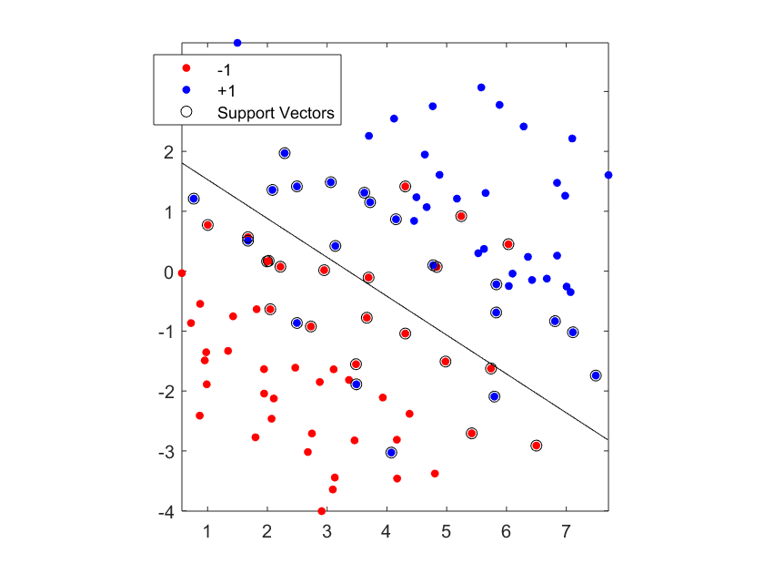
\includegraphics[height=5cm]{pic/linear kernel.png}}
		      \caption{linear kernel示意圖}
		      \label{fig:linear kernel}
	      \end{figure}

	\item
	      Radial Basis Function Kernel
	      \begin{table}[h!]
		      \centering
		      \label{tab:rbf_table}
		      \begin{tabular}{ccc}
\toprule
  & RBF的名字 & 方程式 (\(r = ||\mathbf{c-x_i}||\) )   \\ 
\midrule
  & Gaussian Function  & \(h(x)=\phi(r) = e^{-\varepsilon r}\)      \\ \\ 
  & Linear radial Function  & \(h(x)=\phi(r) = r\)      \\ \\
  & Multiquadric   & \(h(x)=\phi(r) = \sqrt{1+(\varepsilon r)^2}\)       \\ \\
  & Inverse quadric  &  \(h(x)=\phi(r) = \frac{1}{1+(\varepsilon r)^2}\)     \\ \\ 
  & Inverse Multiquadric  &  \(h(x)=\phi(r) = \frac{1}{\sqrt{1+(\varepsilon r)^2}}\)     \\
\bottomrule
\end{tabular}

		      \caption{常見的Radial Basis Function}
	      \end{table}
	      \begin{figure}[H]
		      \centerline{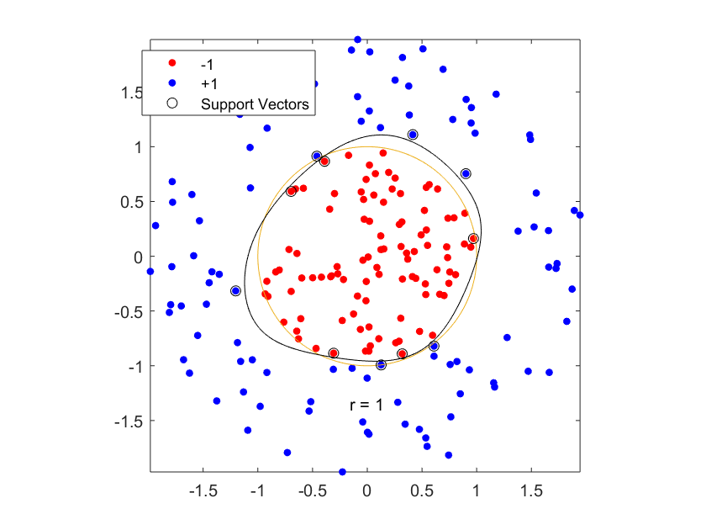
\includegraphics[height=5cm]{pic/Radial Basis Function Kernel.png}}
		      \caption{Radial Basis Function Kernel示意圖}
		      \label{fig:Radial Basis}
	      \end{figure}
	\item
	      Sigmoid Kernel
	      \begin{equation}
		      \label{eqn:Sigmoid Kerne}
		      S(t)=\frac{1}{1+e^{-t}}
	      \end{equation}
	      \begin{figure}[H]
		      \centerline{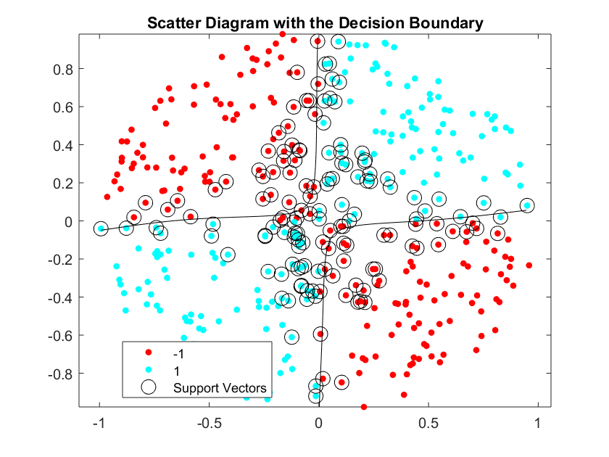
\includegraphics[height=5cm]{pic/Sigmoid Kernel.png}}
		      \caption{Sigmoid Kernel示意圖}
		      \label{Sigmoid Kernel}
	      \end{figure}
\end{enumerate}


\section{結論}
SVM因為是求解最大間隔的超平面,所以能夠得到一個泛化能力較好的模型。更透過與核函數的結合,能夠處理非線性分割的問題。另外也因為SVM有理論推導過程,比起神經網路擁有有較好的可解釋性。

